\documentclass[../Main/main.tex]{subfiles}
\begin{document}
	\chapter{Convergence for MPFA L Method for Elliptic Problems}
	\graphicspath{{../Equivalence between MPFA-L and FEM/figs/}}
	In this chapter we show equivalence between a modified MPFA-L method and a modified finite element method for time dependent problems such as  \eqref{eq:semidiscrete heat}. The challenge of discretizing time dependent, possibly linearized, problems boils down to solving the elliptic problem:
	\begin{equation}\label{eq:stationary_heat}
		\begin{aligned}[c]
		u - \nabla \cdot \pmb{K} \nabla u &= f \\
			u &= 0 \\
			\pmb{K}\nabla u &= g_N
		\end{aligned}
		\ \ \
		\begin{aligned}[c]
			x &\in \Omega  \\
			x &\in  \Gamma_D \\
			x &\in \Gamma_N 
		\end{aligned}
	\end{equation}
	We saw in the section about the MPFA-L method that the interaction regions(L-triangles) may form a triangulation of our domain.
	Modifications are made to both methods so that we can exploit this fact and obtain equivalence. This section is adapted from (Cao, Y., Helmig, R. and Wohlmuth, B.I. (2009),\cite{https://doi.org/10.1002/num.20525})
	\section*{Modified MPFA-L method}
	First of all we assume that we have a parallelogram grid, 
	%\begin{figure}[H]\label{fig:paralellogram mesh}
	%	\centering
	%	%\includegraphics[width=1\textwidth]{paralellogram_mesh.pdf}
	%\end{figure}
	with appropriate boundary conditions and source term.
	As we saw in the previous chapter, one gets with the finite volume method the following relation for all control volumes $\Omega_i$:
	\begin{equation}
		\int_{\Omega_i} u \ dx - \int_{\partial \Omega_i} \pmb{K}\nabla u \cdot \hat{\pmb{n}}\ dx = \int_{\Omega_i} f \ dx
	\end{equation}
	The MPFA-L method deals with the second term, approximating the constitutive law. The other two terms are common to all control volume methods solving time dependent problems or \eqref{eq:stationary_heat} and we will not make modifications or discuss them further.
	\par
	We will need to modify the Neumann boundaries, this is to be expected as finite element methods have degrees of freedom on the boundaries as opposed to finite volume methods. We will also see how we could enforce Dirichlet boundary conditions in a way that is equivalent to the finite element method. On the \textbf{interior} control volumes we use the original MPFA-L method already covered.
	\par
	Consider the control volume $y_1 y_6 y_4 y_3$. 
	\begin{figure}[H]
		\centering
		\includegraphics{modified_L_scheme.pdf}
		\caption{Control volumes in solid lines and interaction regions in dashed lines at the boundary.}
		\label{fig:volemes along boundary}
	\end{figure}
	\begin{figure}[H]
		\centering
		\includegraphics{volumepartition.pdf}
		\caption{Control volume along top boundary.}
		\label{fig:volumepartition}
	\end{figure}
	For the \textbf{Neumann} boundary conditions, we split the cell into two, $y_1 y_6 y_9 y_8$ as $\Omega_2$ and $y_8 y_9 y_4 y_3$ as  $\Omega_1$, see figure \ref{fig:volumepartition} or \ref{fig:volemes along boundary}. For the fluxes on $\Omega_2$ we have six interaction triangles and a normal seven point stencil. For the $\Omega_1$ we compute the flux through $\overline{y_3 y_8}$ using $\triangle x_1 x_3 x_2$, the flux through $\overline{y_8 y_{10}}$ using $\triangle x_1 x_i x_3$, for $\overline{y_{10}y_9}$ and $\overline{y_9 y_4}$ the L triangle  $\triangle x_i x_4 x_3$ is used. Finally the Neumann boundary condition is used at the the edge $\overline{y_4 x_3}$ and $\overline{x_3 y_3}$. We are not able to eliminate the unknown value at $x_3$ and it remains a degree of freedom, which makes sense if we want equivalence with finite element method.
	\par
	In the case of \textbf{Dirichlet} boundary conditions, we compute the fluxes into $y_1 y_6 y_4 y_3$ using seven L-triangles, as can be seen in figure \ref{fig:volemes along boundary}. The flux over the edge $\overline{y_3 y_1}$ are computed as the sum of the flux over $\overline{y_3 y_8}$, $\overline{y_8 y_2}$ and $\overline{y_2 y_1}$ using the L-triangles $\triangle x_1 x_3 x_2$, $\triangle x_1 x_i x_3$ and $\triangle x_1 x_7 x_i$ respectively. Similarly for the edge $\overline{y_6 y_4}$. For $\overline{y_1 y_6}$ we only use the two big L-triangles at the bottom. 
	\par 
	The flux over $\overline{y_4 y_3}$, at the boundary, we compute by balancing it by the other fluxes into the small control volume $\Omega_1$. Let $	q_{\overline{y_i y_j}}:= \int_{\overline{y_i y_j}}  -\pmb{K}\nabla u \cdot \pmb{\hat{n}}\ dx $, then we get
	\begin{equation}\label{eq:K2}
		q_{\overline{y_4 y_3}} =-( q_{\overline{y_3 y_8}} + q_{\overline{y_8 y_{10}}}+q_{\overline{y_{10}y_9}}+q_{\overline{y_9 y_4}}) + \int_{\Omega_1} f \ dx.
	\end{equation}
	
	The fluxes on the right hand side of \eqref{eq:K2} are computed as for the Neumann case.
	\par On the corners we make 
	\section*{Modified finite element method}
	
	In this section we introduce a finite element method for solving \eqref{eq:semidiscrete heat}. We start by observing that by theorem \ref{th:L_triangulation} the L-triangles form a triangulation $\left \{ \tau_h \right \}$. The only modifications we need to make are to the linear form, we let the bi-linear form stay the same as before. We want to define an interpolation operator such that the dot products that make up the linear form become mass conservative in each control volume. We need some notation so that we can distinguish between nodes in the interior, at at cell centers along the boundary and at the boundary. In addition, corner cells introduce edge cases. 
	\par 
	Let $\mathcal{N}_h^*$ be a set of indexes corresponding to all interior nodes of $\left \{ \tau_h \right \}$, which are also the cell centers of the control volume mesh. This index set contains two disjoint sets $\mathcal{N}_h^* = \mathcal{N}_h^b \bigcup \mathcal{N}_h^i$, where superscript $i$ denotes the cell centers of the interior cells and $b$ the boundary cells. $\mathcal{N}^b_h$ are further subdivided as we see in figure \ref{fig:mesWithNodes}. The boundary nodes consists of the set $\mathcal{N}_h^N \bigcup \mathcal{N}_h^D$, where $N$ and $D$ represent neumann and dirichlet boundary nodes. The rest of the notation are explained in figure \ref{fig:mesWithNodes}
	\begin{figure}[H]
		\centering
		\includegraphics{meshWithNodes.pdf}

		\caption{A paralellogram mesh with finite element triangles in dotted lines and control volumes in solid lines. In this case we have a pure Neumann problem.}
		\label{fig:mesWithNodes}
	\end{figure}
	\par 
	As before one denotes by $V_h$ the linear ansatz space, see definition \ref{def:linear ansatz}. Similarly $\phi_i$ is the standard nodal basis function, where $i \in \mathcal{N}_h \setminus \mathcal{N}_h^D$.
	In addition to our global interpolation operator, definition \ref{def:global_interpolator}, we define:
	\begin{definition}[Piecewise global interpolator] \label{def:piecewise_interpolator}
		Let $\hat{I}_h$ be an operator that maps from the test space to functions that are piecewise constant on interior control volumes.
		\begin{equation*}
			\hat{I}_h:C(\Omega)\rightarrow \left \{ v_h \in L^2(\Omega) \right \}
		\end{equation*}
		And
		\begin{equation*}
			\hat{I}_h v = \sum_{i\in \mathcal{N}_h\setminus\mathcal{N}_h^d}v(x_i)\hat{I}_h\phi_i(x)
		\end{equation*}
		Where
		\begin{equation}
			\hat{I}_h\phi_i(x)=\left\{\begin{matrix}
				1 & \text{if } x\in D_i\\ 
				0 & \text{otherwise}
			\end{matrix}\right.
		\end{equation}
		$D_i = \Omega_i$, ie. the corresponding control volume, if $i \in \mathcal{N}_h^i$. If we are close or on the boundary the situation is more complicated: 
		\begin{itemize}
			\item $i \in \mathcal{N}_h^e$: In this case the function vanishes for the quarter of the paralellogram closest to the boundary, ie. $D_i = \Omega_2$ from figure \ref{fig:volumepartition}
			\item $i \in \mathcal{N}_h^{N_e}$ In this case of the neumann boundary node $	\hat{I}_h\phi_i(x)$ vanishes outside the quarter of the control volume closest to the edge, ie. $D_i = \Omega_1$ in figure \ref{fig:volumepartition}
			\item On the corners there are special definitions, see (Cao Wolmuth \cite{https://doi.org/10.1002/num.20525},2009)
		\end{itemize} 
	\end{definition}
	Let $\hat{I}_{\Gamma_N} = \hat{I}_{h}|_{\Gamma_N}$ be the trace of the interpolation operator on the neumann boundary.
	The finite element method we end up with reads as follows: Find $u_h\in V_h$ such that
	\begin{equation} \label{eq:modified_fem}
			\left \langle \hat{I}_h u_h,\hat{I}_h v_h \right \rangle_{0,\Omega} +   \left \langle \pmb{K} \nabla u_h,\nabla v_h \right \rangle_{0,\Omega} = \left \langle f,\hat{I}_h v_h \right \rangle_{0,\Omega} + \left \langle g,\hat{I}_{\Gamma_N} v_h \right \rangle_{0,\Gamma_N},
	\end{equation}
	for all $v_h\in V_h$. 
	The key takeaway here is that the inner products become conservative in the control volumes. This is often referred to as \emph{mass lumping}, see for \cite{baranger1996connection} for examples.  
	\par
		\begin{figure}[H]
		\centering
		\includegraphics[width=1\textwidth]{Control volume.pdf}
		\caption{The support of $\phi_4$}
		\label{fig:control volume}
	\end{figure}
	\begin{figure}[H]
		\centering
		\includegraphics{two triangles.pdf}
		\caption{Notation in the proof}
		\label{fig:two triangles}
	\end{figure}
	Now we can state the equivalence theorem:
	\begin{theorem}
		The modified finite element \eqref{eq:modified_fem} method and the modified MPFA-L method are equivalent on uniform parallelogram grid for the heat equation \eqref{eq:heat equation} on homogenous media. 
	\end{theorem}

	\begin{proof}
		We do the proof in four steps:
		\begin{enumerate}
			\item First we show the equivalence for the interior, so
			let $\Omega_i$ be an interior control volume and $\phi_i$ be the corresponding basis function evaluating to one at the centre of $\Omega_i$, ie. $i \in \mathcal{N}_h^i$.
			Equation \eqref{eq:modified_fem} with $v_h=\phi_i$ then looks like:
			\begin{equation}\label{eq:modified fem interior}
				\left \langle \hat{I}_h u_h,\hat{I}_h \phi_i \right \rangle_{0,\Omega} +   \left \langle \pmb{K} \nabla u_h,\nabla \phi_i \right \rangle_{0,\Omega} = \left \langle f,\hat{I}_h \phi_i \right \rangle_{0,\Omega} .
			\end{equation}
			
			 Let $T \in \tau_h \bigcap \text{supp}(\phi_i)$ be one of the elements in the triangulation that makes up the support of $\phi_i$. $S=T\bigcap \Omega_i$ is a part of the control volume that lies in some element, and $E \subset S\bigcap \partial \Omega_i$ are the half edges of $\Omega_i$. $e$ are the interior edges of $\tau_h$ inside the support of $\phi_i$, see fig \ref{fig:two triangles} and \ref{fig:control volume}. $\pmb{n}_e$ is the unit normal on $e$ with fixed and arbitrary orientation, and $\pmb{n}_E$ is the unit outer normal on $E$. Since $u_h$ and $\phi$ is piecewise linear and $\pmb{\hat{K}}$ is constant on each triangle $T$ we have:
			\begin{equation}\label{eq:big computation}
				\begin{aligned}
					\left \langle \pmb{K}\nabla u_h, \nabla \phi_i \right \rangle_0 &= \int_{\text{supp}(\phi_i)} (\nabla u_h)^T \pmb{K}\nabla \phi_i \ dx = \sum_{T\in \text{supp}(\phi_i)} \int_T (\nabla u_h)^T \pmb{K}\nabla \phi_i \ dx \\
					&= \sum_{T\in \text{supp}(\phi_i)} \left ( \int_{\partial T} (\pmb{K}\nabla u_h)^T \pmb{n}\phi_i \ ds-\int_T \nabla \cdot \pmb{K} \nabla u_h \phi_i \ dx \right ) \\
					&=\sum_{T\in \text{supp}(\phi_i)}\int_{\partial T} (\pmb{K}\nabla u_h)^T \pmb{n}\phi_i \ ds \\
					&= \sum_{e\in \text{supp}(\phi_i)} \int_e ((\pmb{K}\nabla u_h)^T \pmb{n}_e|_{T_{j}} - (\pmb{K}\nabla u_h)^T \pmb{n}_e|_{T_{j+1}})\phi_i \ ds\\
					&= \sum_{e\in \text{supp}(\phi_i)}
					((\pmb{K}\nabla u_h)^T \pmb{n}_e|_{T_{j}} - (\pmb{K}\nabla u_h)^T \pmb{n}_e|_{T_{j+1}}) \frac{|e|}{2}\\
					&=\sum_{S\in \text{supp}(\phi)}\int_{\partial S}  (\pmb{K}\nabla u_h)^T \pmb{n} \ ds - \sum_{E\in \partial \Omega_i}\int_E (\pmb{K}\nabla u_h)^T \pmb{n}_E \ ds\\
					&= \sum_{S\in \text{supp}(\phi)}\int_{ S} \nabla \cdot \pmb{K}\nabla u_h \ ds - \sum_{E\in \partial \Omega_i}\int_E (\pmb{K}\nabla u_h)^T \pmb{n}_E \ ds\\
					&=- \sum_{E\in \partial \Omega_i} (\pmb{K}\nabla u_h)^T \pmb{n}_E |E| 
				\end{aligned}
			\end{equation}
			Note that this last sum is a sum of integrals over the half edges of $\Omega_i$. 
			Further, we have that 
			\begin{equation}\label{eq:mass equiv 1}
				\left \langle \hat{I}_h  u_h,\hat{I}\phi_i \right \rangle_0 = \int_{\Omega}\hat{I}_h u_h \hat{I}_h \phi_i \ dx =  \int_{\Omega_i}u_h(x_i) \ dx
			\end{equation}
			and
			\begin{equation}\label{eq:load equiv 1}
				\left \langle f,\hat{I}_h \phi_i \right \rangle_0 = \int_{\Omega_i}f \ dx.
			\end{equation}
			Combining equation \eqref{eq:big computation}, \eqref{eq:mass equiv 1} and \eqref{eq:load equiv 1} we get that \eqref{eq:modified fem interior} is equivalent to:
			\begin{equation}
				\int_{\Omega_i}u_h(x_i) \ dx - \sum_{E\in \partial \Omega_i} (\pmb{K}\nabla u_h)^T \pmb{n}_E |E| = \int_{\Omega_i}f \ dx.
			\end{equation}
			We know from theorem \ref{lemma:L_potential} that the flux over each half edge in the L-method is given uniquely by the potential values of the three cell centers in the L-triangle. Since the L-triangles and the elements are the same, $\nabla u_h$ corresponds to the gradient used in the L-method, see equation \eqref{eq:L flux simplified}. Hence, if $u$ is the solution to \eqref{eq:stationary_heat} with the original L-method in the interior, then $u(x_i)=u_h(x_i)$ for $x_i\in \mathcal{N}^i_h$. 
			\item For a cell bordering the \textbf{Neumann} boundary, first let $i\in \mathcal{N}_h^e$, we have:
			\begin{equation}\label{eq:case2}
				\left \langle \hat{I}_h u_h,\hat{I}_h \phi_i \right \rangle_{0,\Omega} +   \left \langle \pmb{K} \nabla u_h,\nabla \phi_i \right \rangle_{0,\Omega} = \left \langle f,\hat{I}_h \phi_i \right \rangle_{0,\Omega}.
			\end{equation}
			With similar computations and reasoning as for \eqref{eq:big computation} we get:
			\begin{equation}
					\left \langle \pmb{K} \nabla u_h,\nabla \phi_i \right \rangle_{0,\Omega}= 
					- \sum_{E\in \partial \Omega_{i,2}} (\pmb{K}\nabla u_h)^T \pmb{n}_E |E|, 
			\end{equation}
			where $\Omega_{i,2}$ is as $\Omega_2$ in figure \ref{fig:volumepartition}. As $\hat{I}_h$ is carefully defined close to the Neumann boundary, we get that \eqref{eq:case2} is equivalent to:
			\begin{equation}\label{eq:FVML neumann cell}	\int_{\Omega_{i,2}}u_h(x_i) \ dx - \sum_{E\in \partial \Omega_{i,2}} (\pmb{K}\nabla u_h)^T \pmb{n}_E |E| = \int_{\Omega_{i,2}}f(x_i) \ dx.
			\end{equation}
			Next, let $\hat{i} \in \mathcal{N}_h^{N,e}$, ie the index of a node on the boundary. Then we have 
			\begin{equation}\label{eq:case neumann node}
				\left \langle \hat{I}_h u_h,\hat{I}_h \phi_i \right \rangle_{0,\Omega} +   \left \langle \pmb{K} \nabla u_h,\nabla \phi_i \right \rangle_{0,\Omega} = \left \langle f,\hat{I}_h \phi_i \right \rangle_{0,\Omega}+ \left \langle g,\hat{I}_{\Gamma_N} v_h \right \rangle_{0,\Gamma_N}.
			\end{equation}
			Similarly as in \eqref{eq:big computation} we have:
			\begin{equation}\label{eq:case neumann 1}
				\begin{aligned}
						\left \langle \pmb{K}\nabla u_h, \nabla \phi_{\hat{i}} \right \rangle_0 &= \int_{\text{supp}(\phi_{\hat{i}})} (\nabla u_h)^T \pmb{K}\nabla \phi_{\hat{i}} \ dx = \sum_{T\in \text{supp}(\phi_{\hat{i}})} \int_T (\nabla u_h)^T \pmb{K}\nabla \phi_{\hat{i}} \ dx \\
					&= \sum_{T\in \text{supp}(\phi_{\hat{i}})} \left ( \int_{\partial T} (\pmb{K}\nabla u_h)^T \pmb{n}\phi_{\hat{i}} \ ds-\int_T \nabla \cdot \pmb{K} \nabla u_h \phi_{\hat{i}} \ dx \right ) \\
					&=\sum_{T\in \text{supp}(\phi_{\hat{i}})}\int_{\partial T} (\pmb{K}\nabla u_h)^T \pmb{n}\phi_{\hat{i}} \ ds.
				\end{aligned}
			\end{equation}
			But because $\phi_{\hat{i}}\neq 0$ on $\text{supp}(\phi_{\hat{i}})\bigcap \Gamma_N$, we get
			\begin{equation}\label{eq:case neumann 2}
				\begin{aligned}
					\sum_{T\in \text{supp}(\phi_{\hat{i}})}\int_{\partial T} (\pmb{K}\nabla u_h)^T \pmb{n}\phi_{\hat{i}} \ ds &= \sum_{e\in \text{supp}(\phi_{\hat{i}})} \int_e ((\pmb{K}\nabla u_h)^T \pmb{n}_e|_{T_{j}} - (\pmb{K}\nabla u_h)^T \pmb{n}_e|_{T_{j+1}})\phi_i \ ds\\ &+ \int_{\Gamma_N \bigcap \text{supp}(\phi_{\hat{i}})}(\pmb{K}\nabla u_h)^T \pmb{n}_E \ ds\\
					&= -\sum_{E\in \partial \Omega_{\hat{i}}\setminus \Gamma_N} (\pmb{K}\nabla u_h)^T \pmb{n}_E |E|
				\end{aligned}
			\end{equation}
			Combining \eqref{eq:case neumann 1} and \eqref{eq:case neumann 2} and using the definition of $\hat{I}_h$, definition \ref{def:global_interpolator}, we get that \eqref{eq:case neumann node} is equivalent to:
			\begin{equation}\label{eq:FVML neumann node}
				\int_{\Omega_{\hat{i},1}}u_h(x_i) \ dx - \sum_{E\in \partial \Omega_{\hat{i},1}} (\pmb{K}\nabla u_h)^T \pmb{n}_E |E| = \int_{\Omega_{\hat{i},1}}f(x_i) \ dx.
			\end{equation}
			Where $\Omega_{\hat{i},1}$ is as $\Omega_1$ in figure \ref{fig:volumepartition}. Now, \eqref{eq:FVML neumann cell} and \eqref{eq:FVML neumann node} are exactly the L-method for the Neumann boundary, as described earlier, see figure \ref{fig:volemes along boundary}.  
			\item For a control volume near the \textbf{Dirichlet} boundary, let first $i\in \mathcal{N}_h^e$, ie the cell center. Then, our modified finite element method
			\begin{equation}
				\left \langle \hat{I}_h u_h,\hat{I}_h \phi_i \right \rangle_{0,\Omega} +   \left \langle \pmb{K} \nabla u_h,\nabla \phi_i \right \rangle_{0,\Omega} = \left \langle f,\hat{I}_h \phi_i \right \rangle_{0,\Omega}
			\end{equation}   
			is equivalent to 
			\begin{equation} 
				\int_{\Omega_{i,2}} u_h (x_i) \ dx- \sum_{E\in \partial \Omega_{i,2}} (\pmb{K}\nabla u_h)^T \pmb{n}_E |E| = \int_{\Omega_{i,2}} f \ dx,
			\end{equation} 
			with the same reasoning as in \eqref{eq:big computation}, \eqref{eq:mass equiv 1} and \eqref{eq:load equiv 1}. As $\Omega_i = \Omega_{i,1}\bigcup \Omega_{i,2}$ and $\Omega_{i,1}\bigcap \Omega_{i,2}= \emptyset$, see figure \ref{fig:volumepartition}, we have:
			\begin{equation}
				-\sum_{E\in \Omega_i \setminus \Gamma_D}(\pmb{K}\nabla u_h)^T \pmb{n}_E |E| + \sum_{E\in \Omega_{i,1} \setminus \Gamma_D}(\pmb{K}\nabla u_h)^T \pmb{n}_E |E| + \int_{\Omega_{i,1}} f \ dx = \int_{\Omega_i} f \ dx.
			\end{equation}
			We recognize the second and third terms in the above equation as the flux across the Dirchlet boundary in the modified L method, see \eqref{eq:K2}.
			\item \todo[inline]{Corner cells!}
		\end{enumerate}
	\end{proof}
	\section*{Convergence rate estimates}
	\begin{lemma}[First Lemma of Strang, page 155 \cite{Knabner}]\label{lemma:strang}
		Suppose there exists some $\alpha>0$ such that for all $h>0$ and $v\in V_h$
		\begin{equation*}
			\alpha \left \| v \right \|^2_1 \leq a_h(v,v) 
		\end{equation*}
		and let $a$ be continuous in $V\times V$. Then there exist some constant $C$ independent of $V_h$ such that
		\begin{equation}\label{eq:strang_ineq}
			\left \| u-u_h \right \|_1 \leq C\left \{ \inf_{v \in V_h}\left \{ \left \| u-v \right \|_1 + \sup_{w\in V_h}\frac{|a(v,w)-a_h(v,w)|}{\left \| w \right \|_1}+\sup_{w\in V_h}\frac{|l(w)-l_h(w)|}{\left \| w \right \|_1} \right \} \right \}
		\end{equation}
	\end{lemma}
	From \eqref{eq:modified_fem} we see that our bi-linear form looks like
	\begin{equation}
		a_u(u,v) = \left \langle \hat{I}_h u, \hat{I}_h v \right \rangle_{0,\Omega} +  \left \langle \pmb{K} \nabla u, \nabla v \right \rangle_{0,\Omega} 
	\end{equation}
	And the linear form:
	\begin{equation}
		b_h(v)= \left \langle F,\hat{I}_h v \right \rangle_{0,\Omega} + \left \langle g,\hat{I}_{\Gamma_N} v \right \rangle_{0.\Gamma_N}
	\end{equation}
	To apply the first Lemma of Strang \ref{lemma:strang} we first show that $a_h$ is coercive:
	\begin{equation}
		\begin{aligned}
			\left \| u \right \|_1^2 &= \left \| \partial_{x_1} u \right \|_0^2 + \left \| \partial_{x_2} u \right \|_0^2 + \left \| u \right \|_0^2 \\
			&= \frac{\left \langle \nabla u,\nabla u \right \rangle}{\tau K} + \left \| u \right \|_0^2 \\
			&\leq \frac{\left \langle \nabla u,\nabla u \right \rangle}{\tau K} + C_{\Omega} \left \langle \nabla u, \nabla u \right \rangle \\
			&\leq (\frac{1}{\tau K} + C_{\Omega})(\left \langle \nabla u, \nabla u \right \rangle + \left \langle \hat{I}_h u, \hat{I}_h u \right \rangle)\\
			&\leq \frac{1}{\alpha} a_h(u,u) 
		\end{aligned}
	\end{equation} 
	Another important piece that must be in place for a convergence proof is the piecewise interpolation error:
	\begin{lemma}\label{lemma:int_error}
		For the previously defined piecewise global interpolator $\hat{I}_h$, definition \ref{def:piecewise_interpolator}, we have the estimate:
		\begin{equation}
			\left \| \hat{I}_h u - u \right \|_0 \leq c h | u |_1 \ \forall u \in H^1
		\end{equation}
	\end{lemma}
	\begin{proof}
		\todo[inline]{todo}
		Consider the linear mapping:
		\begin{equation}\label{eq:324}
			\begin{aligned}
				G: H^1(\hat{K})&\rightarrow L^2(\hat{K}) \\
				u &\mapsto \hat{I}_h u - u.
			\end{aligned}
		\end{equation}
		It is continuous by the Sobolev embedding theorem.
		A standard result in functional analysis gives us the estimate:
		\begin{equation}
			\left \| G(v) \right \|_{0,\hat{K}} = \sup \left \{ |\phi (G(v)) |: \phi \in (L^2(\hat{K}))' \text{ and } \left \|\phi \right \|=1 \right \}
		\end{equation}
		For given $\phi$, we have that $\tilde{G}(\cdot) :=\phi(G(\cdot))$ is a continuous linear functional, moreover, $\tilde{G}(q)=0$ for all constant functions $q$. By Bramble Hilbert lemma, we have 
		\begin{equation}
			|\tilde{G}(v)|\leq C \left \| \tilde{G} \right \| |v|_{1,\hat{K}}
		\end{equation}
		Inserting this into \eqref{eq:324}, we obtain:
		\begin{equation}
				\left \| G(v) \right \|_{0,\hat{K}} \leq C \left \| \tilde{G} \right \|  |v|_{1,\hat{K}} \leq C \left \| G \right \| |v|_{1,\hat{K}} \leq C^*|v|_{1,\hat{K}}.
		\end{equation}
		Hence, we have the estimate
		\begin{equation}
			\left \| \hat{I}_h u - u \right \|_{0,\hat{K}} \leq C |u|_{1,\hat{K}},
		\end{equation}
		for some reference element $\hat{K}$.
	\end{proof}

	We are now ready to state the $H^1$ error estimate for the modified finite element method and thus the MPFA-L method:
	\begin{theorem}
		Let $u$ solve \eqref{eq:stationary_heat} and $u_h$ be the solution resulting from MPFA-L , then there exists a positive constant $C$ such that
		\begin{equation}\
			\left \|u_h - u \right \|_1 \leq c h (\left \| u \right \|_2 + \left \| f \right \|_0 + \left \| g \right \|_{\frac{1}{2},\Gamma_N})
		\end{equation}
	\end{theorem}
	\begin{proof}
		The hypothesis in Strang's lemma \ref{lemma:strang} are fulfilled.
		We start by controlling the second term on the right hand side in \eqref{eq:strang_ineq}, the truncation error in the bi-linear form:
		\begin{equation}
			\begin{gathered}
				\sup_{w\in V_h} \frac{|a(v,w)-a_h(v,w)|}{\left \|w \right \|_1} \\
				=\sup_{w\in V_h} \frac{|\left \langle v,w\right \rangle + \tau \left \langle \pmb{K} \nabla v,\nabla w \right \rangle - \left \langle \hat{I}_h v, \hat{I}_h w \right \rangle - \tau \left \langle \pmb{K} \nabla v, \nabla w \right \rangle|}{\left \| w \right \|_1} \\
				=\sup_{w\in V_h} \frac{|\left \langle v,w\right \rangle - \left \langle \hat{I}_h v, w \right \rangle + \left \langle \hat{I}_h v, w \right \rangle - \left \langle \hat{I}_h v, \hat{I}_h w \right \rangle|}{\left \| w \right \|_1}\\
				= \sup_{w\in V_h}\frac{|\left \langle \hat{I}_h v - v,w \right \rangle + \left \langle \hat{I}_h v, \hat{I}_h w - w \right \rangle |}{\left \| w \right \|_1}. \\
			\end{gathered}
		\end{equation}
		We see from the above computations, that the truncation error in the bi-linear form, only has a contribution from the \emph{mass lumping}.
		By Cauchy Schwarz inequality and lemma \ref{lemma:int_error} we get:
		\begin{equation}
			\begin{gathered}
				\leq \sup_{w\in V_h}\frac{Ch\left \| v \right \|_0 | w|_1 + \left \|\hat{I}_h v\right \|_0 Ch|w|_1}{\left \| w \right \|_1}\\
				\leq 				 \sup_{w\in V_h}\frac{Ch\left \| v \right \|_0 | w|_1 + \left \|\hat{I}_h v\right \|_0 Ch|w|_1}{\left \| w \right \|_1} + \frac{ch\left \| v \right \|_0 \left \| w \right \|_0 + \left \|\hat{I}_h v\right \|_0 \left \| w \right \|_0}{\left \| w \right \|_1}\\
				\leq Ch \left (\left \| v \right \|_0 + \left \| \hat{I}_h v \right \|_0 \right ).
			\end{gathered}
		\end{equation}
		The third term, the linear form, can be controlled similarly:
		\begin{equation}\label{eq:334}
			\begin{aligned}
				\sup_{w \in V_h} \frac{l(w)-l_h(w)}{\left \| w \right \|_1} &= \sup_{w \in V_h} \frac{\left \langle f,w-\hat{I}_h w \right \rangle_{0,\Omega} + \left \langle g,w-\hat{I}_{\Gamma_N} w \right \rangle_{0,\Gamma_N}}{\left \| w \right \|_1}\\
				&\leq \sup_{w \in V_h} \frac{\left \|f\right \|_0 Ch\left \|w \right \|_1 + \left \|g\right \|_{\frac{1}{2},\Gamma_N}\left \|w-\hat{I}_{\Gamma_N} w\right \|_{-\frac{1}{2},\Gamma_N}}{\left \| w \right \|_1}.
			\end{aligned}
		\end{equation}
		Now, we want to bound $\left \|w-\hat{I}_{\Gamma_N} w\right \|_{-\frac{1}{2},\Gamma_N}$ by $\left \| w \right \|_1$. Let $v_h$ be piecewise constant functions on the boundary in each Neumann boundary triangle. Then we have:
		\begin{equation}
			\begin{aligned}
				\left \|w-\hat{I}_{\Gamma_N} w\right \|_{-\frac{1}{2},\Gamma_N} &= \sup_{0 \neq v \in H^{\frac{1}{2}}(\Omega)}\frac{\left \langle w-\hat{I}_{\Gamma_N} w,v\right \rangle_{\Gamma_N}}{\left \| v \right \|_{\frac{1}{2},\Gamma_N}}\\
				&=\sup_{0 \neq v \in H^{\frac{1}{2}}(\Omega)}\frac{\left \langle w-\hat{I}_{\Gamma_N} w,v-v_h\right \rangle_{\Gamma_N}}{\left \| v\right \|_{\frac{1}{2},\Gamma_N}},
			\end{aligned}
		\end{equation}
	\todo{What is this inner product?}
		as $\int_{\Gamma_N} (w-\hat{I}_{\Gamma_N} w) \ dx = 0$\todo{Does this make sense?}. Now, we can use Cauchy Schwarz inequality:
		\begin{equation}\label{eq:neumann CS estimate}
			\left \|w-\hat{I}_{\Gamma_N} w\right \|_{-\frac{1}{2},\Gamma_N} \leq \sup_{0 \neq v \in H^{\frac{1}{2}}(\Omega)}\frac{\left \| w-\hat{I}_{\Gamma_N} w\right \|_{0,\Gamma_N}\left \| v-v_h\right \|_{0,\Gamma_N}}{\left \| v\right \|_{\frac{1}{2},\Gamma_N}}.
		\end{equation}
		By the inequality
		\begin{equation}\label{eq:difficult inequality}
			\left \| v-v_h\right \|_{0,\Gamma_N} \leq C h^{\frac{1}{2}} \left \| v \right \|_{\frac{1}{2}, \Gamma_N},
		\end{equation}
		we can bound the right hand side of  \eqref{eq:neumann CS estimate}: 
		\begin{equation}
				\left \|w-\hat{I}_{\Gamma_N} w\right \|_{-\frac{1}{2},\Gamma_N} \leq Ch^{\frac{1}{2}} \left \| w-\hat{I}_{\Gamma_N} w \right \|_{0,\Gamma_N}.
		\end{equation}
		Using \eqref{eq:difficult inequality} again, we get
		\begin{equation}
				\left \|w-\hat{I}_{\Gamma_N} w\right \|_{-\frac{1}{2},\Gamma_N} \leq Ch \left \|w\right \|_{\frac{1}{2},\Gamma_N} \leq Ch\left \| w \right \|_1.
		\end{equation}
		Where the last inequality is due to the definition of the $H^{\frac{1}{2}}$ norm. Inserting this into \eqref{eq:334}, gives us a bound on the truncation error of our linear form:
		\begin{equation}
			\sup_{w \in V_h} \frac{l(w)-l_h(w)}{\left \| w \right \|_1} \leq Ch(\left \|f \right \|_0 + \left \| g \right \|_{\frac{1}{2},\Gamma_N}).
		\end{equation}
		Hence, from \eqref{eq:strang_ineq}, we have the error estimate:
		\begin{equation}\label{eq:341}
					\left \| u - u_h \right \|_1 \leq \inf_{v_h \in V_h}\left \{ \left \| u - v_h \right \|_1 + Ch \left (\left \| v_h\right \|_0 + \left \| \hat{I}_h v_h \right \|_0 + \left \| f \right \|_0 + \left \| g \right \|_{\frac{1}{2},\Gamma_N}\right ) \right \}
		\end{equation}
	If we let $v_h = I_h u \in V_h$ in \eqref{eq:341}, we get the inequality:
	\begin{equation}\label{eq:342}
	\left \| u - u_h \right \|_1 \leq \left \| u - I_h u \right \|_1 + Ch \left (\left \| I_h u\right \|_0 + \left \| \hat{I}_h I_h u \right \|_0 + \left \| f \right \|_0 + \left \| g \right \|_{\frac{1}{2},\Gamma_N} \right )
	\end{equation}
	As discussed earlier, in section \ref{sec:convergence} about convergence of finite element method, we have the estimate:
	\begin{equation}
 \left \| u - I_h u \right \|_1 \leq C h|u|_2.
	\end{equation}
	If we insert this into \eqref{eq:342}, we get:
	\begin{equation}
	\left \| u - u_h \right \|_1 \leq  Ch \left ( |u|_2 + \left \| I_h u\right \|_0 + \left \| \hat{I}_h I_h u \right \|_0 + \left \| f \right \|_0 + \left \| g \right \|_{\frac{1}{2},\Gamma_N} \right ).
	\end{equation}
	As $I_h u, \hat{I}_h u \rightarrow u$ as $h\rightarrow 0$, we can control the first three terms inside the parenthesis by the $H^2$ norm of $u$, and we get the desired result:
	\begin{equation}
\left \| u - u_h \right \|_1 \leq  Ch \left ( \left \|u\right \|_2 + \left \| f \right \|_0 + \left \| g \right \|_{\frac{1}{2},\Gamma_N} \right ).	\end{equation}
	\end{proof}
\end{document}